\chapter{Lane Following}
\section{Lane Following System}
\subsection{Problem Formulation}
A lane-following system is a control system that keeps the vehicle traveling along the centerline of a highway lane, while maintaining a user-set velocity. Figure \ref{fig:laneFollowing} illustrates a typical lane following scenario.
\begin{figure}[!h]
	\centering
	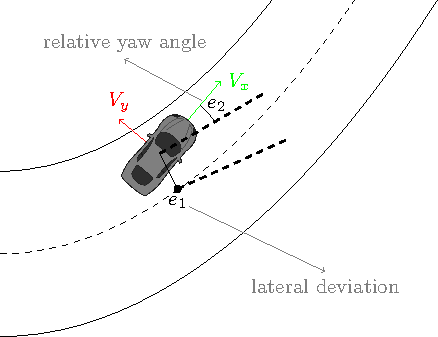
\includegraphics[width=0.75\textwidth]{../figure/laneFollowing/laneFollowing.pdf}
	\caption{Problem description of a lane following system.}
	\label{fig:laneFollowing}
\end{figure}
In a classic lane keeping assist, it is assumed that the longitudinal velocity is constant \cite{borelli3}. This restriction is relaxed in this model because the longitudinal acceleration varies in this MIMO control system. This lane-following system manipulates both the longitudinal acceleration and the front steering angle of the vehicle to keep the lateral deviation and the relative yaw angle small and the longitudinal velocity close to a driver set velocity. If these two goals cannot be met at the same moment, the system tries to balance them. The model that we are considering contains many parameters. The first fundamental block describes the vehicle dynamics: we have applied the bicycle model of lateral vehicle dynamics and approximate the longitudinal dynamics using a time constant obtaining  a linear model.
\subsubsection{Longitudinal dynamics}
We can use the following state space to describe the longitudinal model:
\begin{equation}
\label{eqn:longi_dynamics_simple_model_ss}
\begin{array}{ll}
\dot{\vec{x}}_{\text{lon}} =\vec{A}_m \vec{x}_{\text{lon}}+ \vec{B_m}\vec{u}_{\text{lon}}\\
\vec{y}_{\text{lon}} =\vec{C_m} \vec{x}_{\text{lon}} + \vec{D_m} \vec{u}_{\text{lon}}
\end{array}
\end{equation}
where the input is the acceleration and the states are the longitudinal velocity and the actual acceleration which is also the only output of this system.
\begin{equation}
\vec{x}_{\text{lon}} = \begin{bmatrix}
\dot{V}_x\\V_x
\end{bmatrix},
\qquad
\vec{u}_{\text{lon}} = a
\end{equation}
and
\begin{equation}
\begin{array}{cc}
\vec{A_m}=\begin{bmatrix}
-\frac{1}{\tau}&0\\1&0
\end{bmatrix},
\qquad
\vec{B_m}=\begin{bmatrix}
\frac{1}{\tau}\\
0
\end{bmatrix},\\\\
\vec{C_m}=\begin{bmatrix}
1&0
\end{bmatrix}, 
\qquad
\vec{D_m}=0.
\end{array}
\end{equation}
where $\tau$ is a time constant \cite{long_tf}; in practice we are considering a second order transfer function like in \cite{longitudinal}.
\subsubsection{Lateral dynamics}
Local function: we have a continuous vehicle lateral model from parameters obtained by simplifying the one in \cite{rathai}: 
\begin{equation}
\label{eqn:lateral_dynamics_simple_model}
\begin{array}{ll}
\dot{\vec{x}}_{\text{lat}} =\vec{A}_g \vec{x}_{\text{lat}}+ \vec{B}_g \vec{u}_{\text{lat}}\\
\vec{y}_{\text{lat}} =\vec{C}_g \vec{x}_{\text{lat}} + \vec{D}_g \vec{u}_{\text{lat}}
\end{array}
\end{equation}
where the input is the steering angle in radians, and the outputs are the lateral velocity in meters per second and yaw angle rate in radians per second:
\begin{equation}
\vec{x}_{\text{lat}} = \begin{bmatrix}
V_y\\\dot{\psi}
\end{bmatrix}
\qquad
\vec{u}_{\text{lat}} = \delta
\end{equation}
and
\begin{equation}
\begin{array}{cc}
\vec{A}_g=
\begin{bmatrix}
\displaystyle -\frac{2C_F+2C_R}{mV_x}&\displaystyle -\frac{2C_Fl_F-2C_Rl_R}{mV_x} - V_x\\
\displaystyle -\frac{2C_Fl_F-2C_Rl_R}{I_ZV_x}&\displaystyle -\frac{2C_Fl_F^2+2C_Rl_R^2}{I_ZV_x}
\end{bmatrix},
\\\\
\vec{B}_g=\begin{bmatrix}
2C_F/m\\2C_Fl_F/I_Z
\end{bmatrix},
\qquad
\vec{C}_g=\begin{bmatrix}
1&0\\0&1
\end{bmatrix}=
\vec{I}_2, 
\qquad
\vec{D}_g=\begin{bmatrix}
0\\0
\end{bmatrix}=
\vec{0}_{2\times1}.
\end{array}
\end{equation}
The parameters in the previous matrices are:
\begin{itemize}
	\item $V_x$ is the longitudinal velocity of the car;	
	\item $m$ is the total mass parameter; 
	\item $I_Z$ is the yaw moment of inertia parameter;
	\item $l_F$ and $l_R$ are the longitudinal distances from center of gravity to front and rear tires parameters;
	\item $C_F$ and $C_R$ are the cornering stiffnesses of front and rear tires parameters.
\end{itemize}
The goal for the driver steering model is to keep the vehicle in its lane and follow the curved road by controlling the front steering angle . This goal is achieved by driving the yaw angle error $e_2 = \psi -\psi_{\text{des}}$ and lateral displacement error $e_1$ to zero ($\dot{e}_1 = V_xe_2+V_y$). We can incorporate these two paramenters in the augmented model:
\begin{equation}
\label{eqn:lateral_dynamics_augmented_model}
\begin{array}{ll}
\dot{\vec{x}}_{\text{aug}} =\vec{A}_a \vec{x}_{\text{aug}}+ \vec{B}_a \vec{u}_{\text{aug}}\\
\vec{y}_{\text{aug}} = \vec{C}_a \vec{x}_{\text{aug}} + \vec{D}_a \vec{u}_{\text{aug}}
\end{array}
\end{equation}
where
\begin{equation}
\vec{x}_{\text{aug}} = \begin{bmatrix}
V_y\\\dot{\psi}\\e_1\\e_2
\end{bmatrix},
\qquad
\vec{u}_{\text{aug}} = 
\begin{bmatrix}
\delta\\\dot{\psi}_{\text{des}}
\end{bmatrix}
\end{equation}
and
\begin{equation}
\begin{array}{cc} 
\vec{A}_a=\begin{bmatrix}
\vec{A}_g&\vec{0}_{2\times2}\\
\vec{I}_2&\begin{matrix}
0&V_x\\
0&0
\end{matrix}
\end{bmatrix},
\qquad
\vec{B}_a=\begin{bmatrix}
\vec{B}_g&\vec{0}_{2\times1}\\
0&0\\
0&-1
\end{bmatrix},
\\\\
\vec{C}_a=\begin{bmatrix}
\vec{0}_{2\times2}&\vec{I}_2
\end{bmatrix}, 
\qquad
\vec{D}_a=
\vec{0}_{2\times2}. 
\end{array}
\end{equation}

Combining (\ref{eqn:longi_dynamics_simple_model_ss}) with (\ref{eqn:lateral_dynamics_augmented_model}) yields the state-space model that characterizes the Model Predictive Controller:
\begin{equation}
\label{eqn:full_dynamics_model}
\begin{array}{ll}
\dot{\vec{x}}_{\text{tot}} = \vec{A}_f \vec{x}_{\text{tot}}+ \vec{B}_f \vec{u}_{\text{tot}}\\
\vec{y}_{\text{tot}} = \vec{C}_f \vec{x}_{\text{tot}} + \vec{D}_f \vec{u}_{\text{tot}}
\end{array}
\end{equation}
where
\begin{equation}
\vec{x}_{\text{tot}} = \begin{bmatrix}
\vec{x}_{\text{lon}}\\\vec{x}_{\text{aug}}
\end{bmatrix} = \begin{bmatrix}
\dot{V}_x\\V_x\\V_y\\\dot{\psi}\\e_1\\e_2
\end{bmatrix},
\qquad
\vec{u}_{\text{tot}} = \begin{bmatrix}
\vec{u}_{\text{lon}}\\\vec{u}_{\text{aug}}
\end{bmatrix}  =
\begin{bmatrix}
a\\\delta\\\dot{\psi}_{\text{des}}
\end{bmatrix}
\end{equation}
and
\begin{equation}
\begin{array}{cc}
\vec{A}_f=\begin{bmatrix}
\vec{A}_m&\vec{0}_{2\times4}\\
\vec{0}_{4\times2}&\vec{A}_a
\end{bmatrix},
\qquad
\vec{B}_f=\begin{bmatrix}
\vec{B}_m&\vec{0}_{2\times2}\\
\vec{0}_{4\times1}&\vec{B}_a
\end{bmatrix},
\\\\
\vec{C}_f=\begin{bmatrix}
\vec{C}_m&\vec{0}_{1\times4}\\
\vec{0}_{2\times2}&\vec{C}_a
\end{bmatrix}, 
\qquad
\vec{D}_f=\vec{0}_{3\times3}. 
\end{array}
\end{equation} 

However the system to be controlled is usually modeled by a linear discrete state-space model:
\begin{equation}
\label{eqn:full_dynamics_model_disc}
\begin{array}{rr}
{\vec{x}}_{\text{tot}}(k+1) =\vec{A} \vec{x}_{\text{tot}}(k)+ \vec{B} \vec{u}_{\text{tot}}(k)\\
\vec{y}_{\text{tot}}(k) = \vec{C}\vec{x}_{\text{tot}}(k) + \vec{D} \vec{u}_{\text{tot}}(k)
\end{array}
\end{equation}
where $\vec{A}$ and $\vec{B}$ are the state and control matrices for the discrete state-space equation, respectively, which can be calculated, also in this case, with the Euler method as:
\[
\vec{A} = e^{\vec{A}_fT_s},\qquad \vec{B} = \int_{kT_s}^{(k+1)T_s} e^{\vec{A}_f[(k+1)T_s-\eta]}\vec{B}_f d\eta
\]
where $T_s$ is the sampling interval for the discrete state-space model. The matrices $\vec{C}$ and $\vec{D}$ are equivalent to those in the continuous case.

\subsection{Design of Adaptive Model Predictive Control}
We created an Adaptive MPC controller with a prediction model that has six states, three outputs (longitudinal velocity, lateral deviation, relative yaw angle), and two manipulated signals (acceleration and steering). 
The objective of the trajectory planning along specified path can be described as follows: given a path which the vehicle is expected to follow design a trajectory of a car-vehicle configuration.
In order to do this, according with \cite{curvature} it is possible to derive the road curvature and its derivative.
The product of the road curvature and the longitudinal velocity is modeled as a measured disturbance. We have set the constraints for manipulated variables and the scale factors. Moreover we have specified the weights in the standard MPC cost function. The third output, yaw angle, is allowed to float because there are only two manipulated variables to make it a square system. In this controller, there is no steady-state error in the yaw angle as long as the second output, lateral deviation, reaches 0 at steady state. Finally we have also penalized acceleration change more for smooth driving experience. This controller uses a linear model for the vehicle dynamics and updates the model online as the longitudinal velocity varies.

\subsection{Simulation Results}
The proposed adaptive MPC algorithm is designed in the MATLAB/Simulink and validated through simulation. The objective of this test is to evaluate the behavior of the proposed control strategy in critical situations.
Table 3 shows the parameters used in the lane following simulation.
\begin{table}[!h]
	\centering
	\begin{tabular}{|c|c|}
		\hline
		Parameters          & Values      \\
		\hline
		$m$          & \SI{1575}{kg}              \\
		$I_z$         & \SI{2875}{kgm^2}               \\
		$l_F$           & \SI{1.2}{m}               \\
		$l_R$         & \SI{1.6}{m}               \\
		$C_F$          & \SI{19000}{\newton/rad}      \\
		$C_R$           & \SI{33000}{\newton/rad}  \\
		$\tau$             & 0.2                \\
		$V_0$           & \SI{15}{m/s}       \\
		$V_{\text{set}}$          & \SI{20}{m/s}   \\
		$T_s$         & \SI{0.02}{s}          \\
		\hline
	\end{tabular}
\end{table}

Figures \ref{fig:reference_laneFollowing} and \ref{fig:curvature_laneFollowing} show the desired path that the car must follow and its curvature, where the former is described in terms of the lateral position $Y_{\text{ref}}$ as function of the longitudinal position $X_{\text{ref}}$ and the latter is derived according with \cite{curvature}. The ATLASCAR2 is controlled to follow a sinusoidal trajectory which is given as follows:
\begin{equation*}
X_\text{ref}=V_x\cdot t, \quad Y_\text{ref}=5\sin(X_\text{ref}/20)\quad \text{with}\quad t\in[0,20]\SI{}{s}
\end{equation*}
\begin{figure}[!t]
	\centering
	\begin{minipage}[t]{0.49\textwidth}
		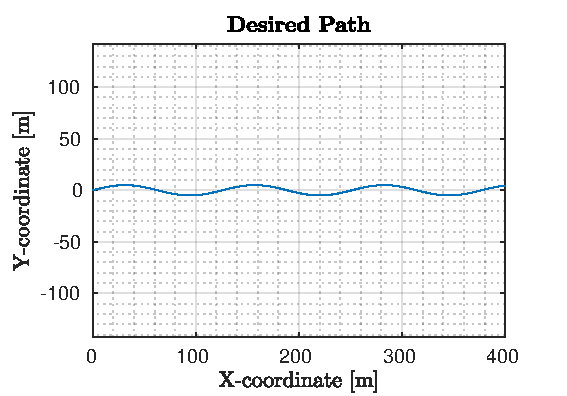
\includegraphics[width=\textwidth]{../../MATLAB/lane_following/figure/Reference.pdf}
		\subcaption{}
		\label{fig:reference_laneFollowing}
	\end{minipage}
	\begin{minipage}[t]{0.5\textwidth}
		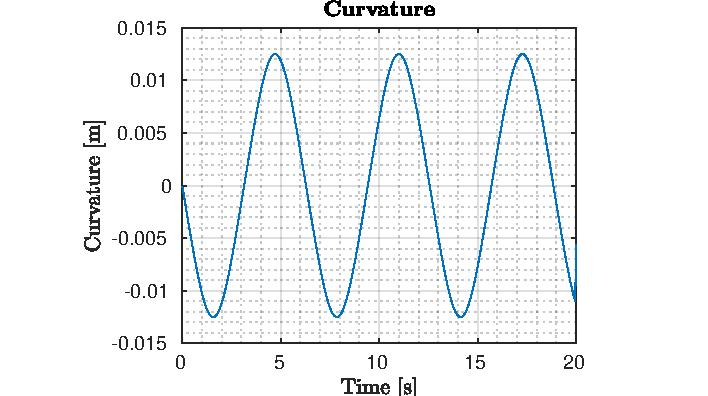
\includegraphics[width=\textwidth]{../../MATLAB/lane_following/figure/Curvature.pdf}
		\subcaption{}
		\label{fig:curvature_laneFollowing}
	\end{minipage}
	\caption{Desired path and curvature of the ATLASCAR2 in a simulation of \SI{20}{s}}
	\label{fig:laneFollowing_desired}
\end{figure}

Moreover the following figures show the trend of the main parameters confirming that the control strategy used allows the vehicle to follow the path. In particular we simulated also a small error in the sensor dynamics in order to make the simulation more realistic: we added a 3 percent error to the longitudinal velocity and this is evident from the small noise in the graphs of the steering angle (Fig.\ref{fig:steering_laneFollowing}) and the lateral deviation (Fig.\ref{fig:lateral_deviation_laneFollowing}).
Figure {\ref{fig:longitudinal_velocity_laneFollowing}} shows the evolution of the vehicle longitudinal velocity. At the start of the simulation, this velocity is equal to the initial condition for longitudinal velocity parameter $V_0$. At run time, we can note that $V_x$ reaches the predefined value of \SI{20}{m/s} meters for second and then it stabilizes near the cruising speed because it continues to vary the steering angle to adapt to the path to be followed. Finally we presents the overall scheme for the lane following developted in Simulink depicted in Figure \ref{fig:scheme_lane_following}.
\begin{figure}[!h]
	\centering
	\begin{minipage}[t]{0.49\textwidth}
		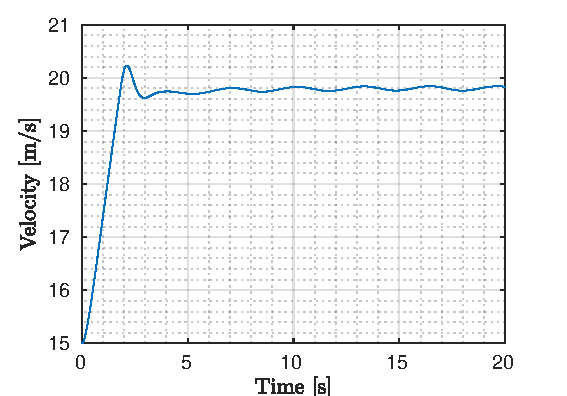
\includegraphics[width=\textwidth]{../../MATLAB/lane_following/figure/LongitudinalVelocityVsTime.pdf}
		\subcaption{Longitudinal velocity $V_x$ with respect to time.}
		\label{fig:longitudinal_velocity_laneFollowing}
	\end{minipage}
	\begin{minipage}[t]{0.49\textwidth}
		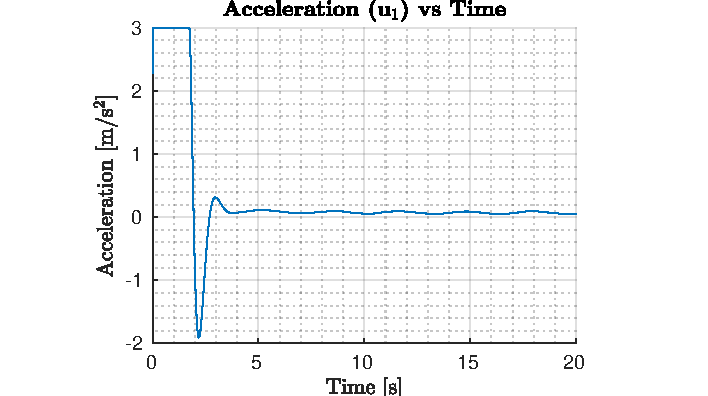
\includegraphics[width=\textwidth]{../../MATLAB/lane_following/figure/AccelerationVsTime.pdf}
		\subcaption{Acceleration $u_1$ with respect to time.}
		\label{fig:acceleration_laneFollowing}
	\end{minipage}
	\begin{minipage}[t]{0.49\textwidth}
		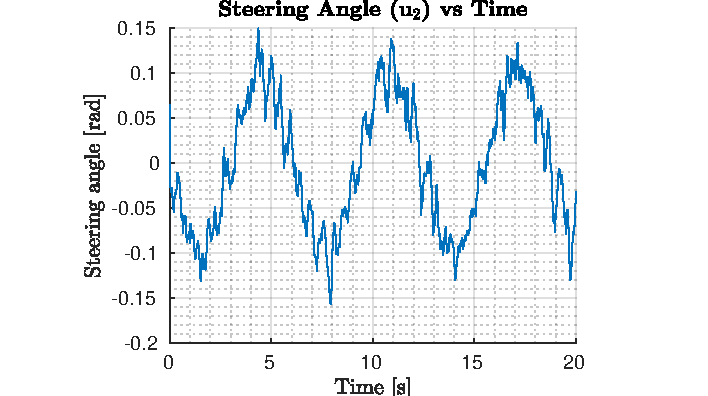
\includegraphics[width=\textwidth]{../../MATLAB/lane_following/figure/SteeringAngleVsTime.pdf}
		\subcaption{Steering angle $u_2$ with respect to time.}
		\label{fig:steering_laneFollowing}
	\end{minipage}
	%\begin{minipage}[t]{\columnwidth}
	%	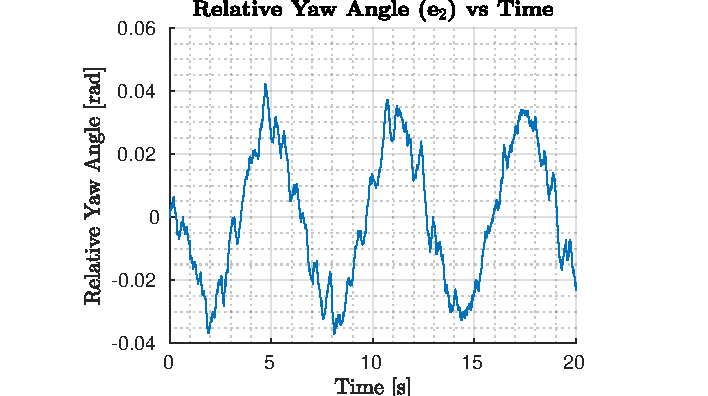
\includegraphics[width=\columnwidth]{../../MATLAB/lane_following/figure/RelativeYawAngleVsTime.pdf}
	%	\subcaption{Relative yaw angle $e_2$ with respect to time.}
	%	\label{fig:relative_yaw_angle_laneFollowing}
	%\end{minipage}
	\begin{minipage}[t]{0.49\textwidth}
		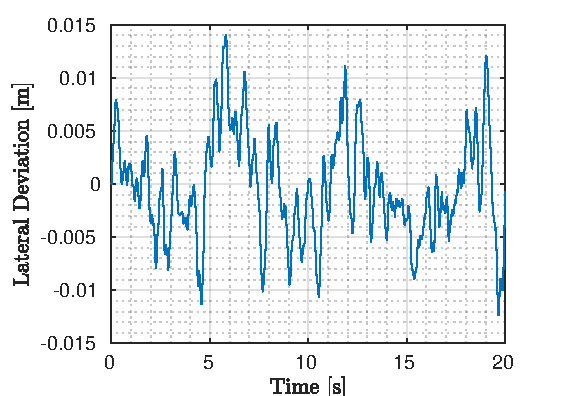
\includegraphics[width=\textwidth]{../../MATLAB/lane_following/figure/LateralDeviationVsTime.pdf}
		\subcaption{Lateral deviation $e_1$ with respect to time.}
		\label{fig:lateral_deviation_laneFollowing}
	\end{minipage}
	\caption{Time signals of the ATLASCAR2 in the simulation with a sinusoidal path.}
	\label{fig:laneFollowing_signals}
\end{figure}

\begin{figure}[!h]
	\centering
	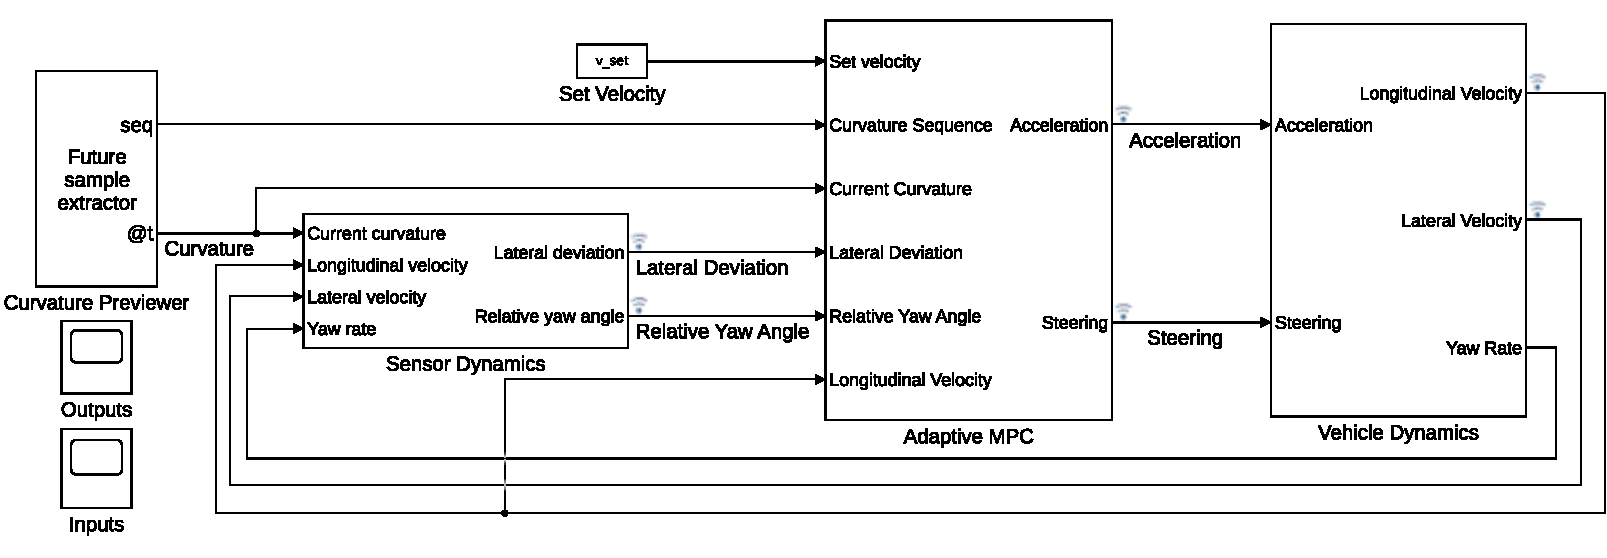
\includegraphics[width=\textwidth]{../figure/lane_following_AMPC.pdf}
	\caption{Overall procedure scheme lane following.}
	\label{fig:scheme_lane_following}
\end{figure}

%%%CIAOOOOOOOOOOOOOOOOOOOOOOOOOOOOOOOOOOOOOOOOOO

